\documentclass[letterpaper,11pt,twocolumn]{article}
\usepackage{amsmath}
\usepackage{usenix,graphicx,times}
\usepackage{hyperref}
\usepackage{subcaption}
\usepackage{pgfplots, pgfplotstable}
\usepgfplotslibrary{statistics}

\usepackage{tikz}
\usetikzlibrary{matrix,positioning,calc,arrows,decorations.pathreplacing}
\usepackage{tikzscale}

\usepackage{outlines}
\usepackage{titling}

\newcommand{\code}[1]{\texttt{\small #1}}
\setlength{\fboxsep}{0pt}
\newcommand{\hl}[1]{\colorbox{black!20}{#1}}



% taken from manual
\makeatletter
\pgfdeclareshape{document}{
\inheritsavedanchors[from=rectangle] % this is nearly a rectangle
\inheritanchorborder[from=rectangle]
\inheritanchor[from=rectangle]{center}
\inheritanchor[from=rectangle]{north}
\inheritanchor[from=rectangle]{south}
\inheritanchor[from=rectangle]{west}
\inheritanchor[from=rectangle]{east}
% ... and possibly more
\backgroundpath{% this is new
% store lower right in xa/ya and upper right in xb/yb
\southwest \pgf@xa=\pgf@x \pgf@ya=\pgf@y
\northeast \pgf@xb=\pgf@x \pgf@yb=\pgf@y
% compute corner of ??flipped page??
\pgf@xc=\pgf@xb \advance\pgf@xc by-10pt % this should be a parameter
\pgf@yc=\pgf@yb \advance\pgf@yc by-10pt
% construct main path
\pgfpathmoveto{\pgfpoint{\pgf@xa}{\pgf@ya}}
\pgfpathlineto{\pgfpoint{\pgf@xa}{\pgf@yb}}
\pgfpathlineto{\pgfpoint{\pgf@xc}{\pgf@yb}}
\pgfpathlineto{\pgfpoint{\pgf@xb}{\pgf@yc}}
\pgfpathlineto{\pgfpoint{\pgf@xb}{\pgf@ya}}
\pgfpathclose
% add little corner
\pgfpathmoveto{\pgfpoint{\pgf@xc}{\pgf@yb}}
\pgfpathlineto{\pgfpoint{\pgf@xc}{\pgf@yc}}
\pgfpathlineto{\pgfpoint{\pgf@xb}{\pgf@yc}}
\pgfpathlineto{\pgfpoint{\pgf@xc}{\pgf@yc}}
}
}
\makeatother

\tikzstyle{doc}=[%
draw,
thick,
align=center,
color=black,
shape=document,
minimum width=12mm,
minimum height=16mm,
inner sep=2ex,
]




\begin{document}

\title{Public Record: Implementing a Real-Time Collaborative Editor 
Using Operational Transformation}
\date{}

\author{
  {\rm Jonas Luebbers}\hspace{1cm}
  {\rm David Moon}
}

\maketitle

\thispagestyle{empty}
%\pagestyle{empty}
                                   
\section{Introduction}

This paper presents our implementation of Public Record, a publicly accessible real-time collaborative document editor.  Public Record maintains a single, persistent, unbounded document.  Users may read and edit this document through a minimal web interface consisting of a single text box, which is accessible by any bored individual with the URL and nothing better to do.  The purpose of this project was to learn about and implement a general technique for optimistic concurrency control called Operational Transformation (OT).

We begin in Section \ref{sec:background} with an overview of the particular requirements imposed by real-time collaboration and the key concepts underlying OT; we also review and compare against OT some recently developed, alternative solutions for  optimistic concurrency control.  We then describe in Section \ref{sec:architecture} our implementation of OT in Public Record; we also describe in this section a number of other key features, optimizations, and challenges encountered during development.  In Section \ref{sec:evaluation}, we evaluate the performance of Public Record.  Finally, in Section \ref{sec:future}, we discuss various directions for future work.



%Unfortunately, implementing OT sucks. There's a million algorithms with different tradeoffs, mostly trapped in academic papers. The algorithms are really hard and time consuming to implement correctly. ... Wave took 2 years to write and if we rewrote it today, it would take almost as long to write a second time.

\section{Background} \label{sec:background}

\paragraph*{Real-time collaboration}
The complexity of real-time collaborative editors (RTCEs) stems from a fundamental tension between (1) the standard of developing a smooth user experience and (2) the reality of network latency.  Users should be able to edit the same document simultaneously and at will; in particular, for the user experience to be sensible, each should see her own edits be applied immediately.  With network latency, this rules out a simple lock-based approach in which users pass back and forth an ``edit document'' token while applying edits to a single central document.  Immediate updates can only be applied locally, and thus an RTCE must manage multiple user-local copies that are being updated concurrently.  As these copies represent the same document, an RTCE must also ensure that they eventually converge. 
\begin{figure}
\centering
	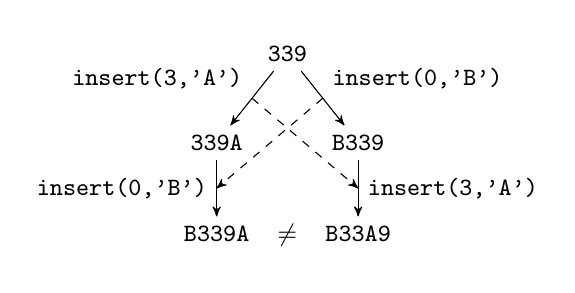
\begin{tikzpicture}[>=stealth',font=\ttfamily\small]
		\matrix (m) [
			matrix of nodes,
			row sep=2em,
			column sep=0em,
		]
		{
			& \node (go) {339}; & \\
			\node (goa) {339A}; & & \node (got) {B339}; \\
			\node (gota) {B339A}; & $\not=$ & \node (goat) {B33A9};\\
		};
		\path[->]
			(go) edge[above left]  node {insert(3,'A')} (goa)
				 edge[above right] node {insert(0,'B')} (got)
			(goa) edge[left]  node {insert(0,'B')} (gota)
			(got) edge[right] node {insert(3,'A')} (goat)
		;
		\path[->,dashed]
			($ (go)!1.0/2!(goa) $) edge ($ (got)!1.0/2!(goat) $)
			($ (go)!1.0/2!(got) $) edge ($ (goa)!1.0/2!(gota) $)
		;

%		\path[<-]
%			(??) edge[below left]  node {insert(2,'t')} (goa)
%				 edge[below right] node {insert(2,'a')} (got)
%		;
	\end{tikzpicture}
\caption{No convergence due to noncommutativity.}
\label{fig:noncommutative}
\end{figure}


\newcommand{\xra}[1]{\xrightarrow{#1}}
\newcommand{\tcode}[1]{\texttt{\footnotesize #1}}
The raises a new problem: edits may be noncommutative.  Suppose Alice and Bob are collaborating on a document that currently reads \code{339} on both of their local copies.  Alice applies the operation \code{insert(3,'A')}, which updates her local copy to \code{339A}.  Simultaneously, Bob applies the operation \code{insert(0,'B')}, updating his local copy to \code{B339}.  Upon receiving each other changes, Alice and Bob cannot both simply apply them verbatim.  If they did, Alice's local copy would follow the left branch in Figure \ref{fig:noncommutative} and arrive at \code{B339A}, while Bob's local copy would follow the right branch and arrive at \code{B33A9}.  That is, their local copies would not converge.



\paragraph*{Operational Transformation}
One solution to this issue is Operational Transformation.  OT is a general technique for optimistic concurrency control that is widely used today in real-world systems such as Apache Wave and Google Docs.  OT incorporates domain-specific knowledge of the state space at hand in order to resolve the issue of noncommutativity such as that encountered by Alice and Bob above.

At the heart of OT is the \emph{transform} function, denoted by \code{xform}, which takes operations performed in one context and transforms them to apply in another.  The \code{xform} function takes a pair $(p,q)$ of operations concurrently applied to some common \code{state} and produces a new pair $(p',q')$ of operations such as that
\begin{align*}
	&\small\texttt{state.apply$(p)$.apply$(q')$} \\
	=\ \ &\small\texttt{state.apply$(q)$.apply$(p')$}.
\end{align*}
This is visually captured by the diamond-shaped schematic in Figure \ref{fig:transform}.
The \code{xform} function is symmetric in the sense that, if $\code{xform}(p,q) = (p',q')$ and $\code{xform}(q,p) = (q'',p'')$, then $p' = p''$ and $q' = q''$.
%The \code{xform} function is defined under the assumption that $o_1$ was locally applied before $o_2$ was locally applied.

\begin{figure}
\centering
	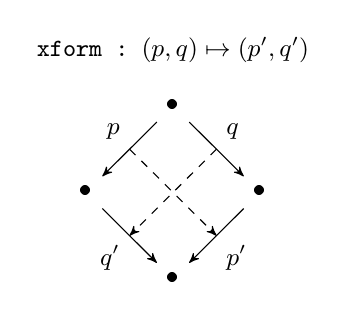
\begin{tikzpicture}[>=stealth',font=\ttfamily\small]
		\node (fn) {xform :\ $(p,q)\mapsto(p',q')$};
	
		\matrix (m) [
			below=.1 of fn,
			matrix of nodes,
			row sep=2em,
			column sep=2em,
		]
		{
			& \node (go) {\textbullet}; & \\
			\node (goa) {\textbullet}; & & \node (got) {\textbullet}; \\
			&  \node (goat) {\textbullet}; & \\
		};
		\path[->]
			(go) edge[above left]  node {$p$} (goa)
				 edge[above right] node {$q$} (got)
		;
		\path[<-]
			(goat) edge[below left]  node {$q'$} (goa)
				   edge[below right] node {$p'$} (got)
		;
		\path[->,dashed]
			($ (go)!1.0/2!(goa) $) edge ($ (got)!1.0/2!(goat) $)
			($ (go)!1.0/2!(got) $) edge ($ (goa)!1.0/2!(goat) $)
		;
	\end{tikzpicture}
\caption{The \code{xform} function.}
\label{fig:transform}
\end{figure}

The use of the \code{xform} function in the case of document editing with Alice and Bob is displayed in Figure \ref{fig:ot}.  
%Here, we assume that Alice and Bob are both aware that Alice's operation was applied before Bob's; how they determine this is orthogonal to OT and described in Section \ref{sec:architecture}.    
Upon receiving Bob's operation \code{insert(0,'B')}, Alice transforms it against her locally applied operation \code{insert(3,'A')} and applies the result \hl{\code{insert(0,'B')}}; in this case, the transformed result is the same as the original operation because Alice's local operation occurred later within the document string and therefore has no effect on Bob's operation index.  Symmetrically, upon receiving Alice's operation \code{insert(3,'A')}, Bob transforms it against his locally applied operation \code{insert(0,'B')} and applies the result \hl{\code{insert(4,'A')}}; in this case, the transformed result takes into account the index change imposed by Bob's local operation.  
\begin{figure}
\centering
\setlength\tabcolsep{2pt}
	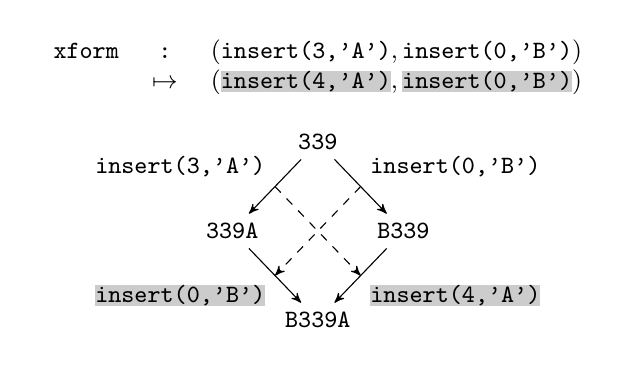
\begin{tikzpicture}[>=stealth',font=\ttfamily\small]
		\node (fn) {
			\begin{tabular}{ccc}
			xform & : & $(\code{insert(3,'A')},\code{insert(0,'B')})$ \\
			& $\mapsto$ & $(\hl{\code{insert(4,'A')}},\hl{\code{insert(0,'B')}})$
			\end{tabular}
		};
	
		\matrix (m) [
			below=.1 of fn,
			matrix of nodes,
			row sep=2em,
			column sep=.3em,
		]
		{
			& \node (go) {339}; & \\
			\node (goa) {339A}; & & \node (got) {B339}; \\
			&  \node (goat) {B339A}; & \\
		};
		\path[->]
			(go) edge[above left]  node {insert(3,'A')} (goa)
				 edge[above right] node {insert(0,'B')} (got)
		;
		\path[<-]
			(goat) edge[below left]  node {\hl{insert(0,'B')}} (goa)
				   edge[below right] node {\hl{insert(4,'A')}} (got)
		;
		\path[->,dashed]
			($ (go)!1.0/2!(goa) $) edge ($ (got)!1.0/2!(goat) $)
			($ (go)!1.0/2!(got) $) edge ($ (goa)!1.0/2!(goat) $)
		;
	\end{tikzpicture}
\caption{Convergence via OT.}
\label{fig:ot}
\end{figure}

Altogether, this ensures that both Alice and Bob's local copies converge to the state \code{B339A}.  The \texttt{xform} function may also have been defined such that their copies converge to \code{B33A9} (cf.\ Figure \ref{fig:noncommutative}); which final state is chosen for convergence, however, is not important.

%Finally, note that the \code{xform} function may be lifted to sequences of operations in a well-defined manner, as shown in Figure \ref{fig:lift-to-seq}.  Thus, if Bob had applied two operations at the same time as Alice's operation, he may 

%\begin{figure}
%\centering
%	\begin{tikzpicture}[>=stealth',font=\small\ttfamily]
%		\node (fn) {
%			xform :\ $(p,q_1q_2)\mapsto(p'',q'_1q'_2)$ 
%%			\begin{tabular}{ccc}
%%			xform & : & $(p,q_1q_2)$ \\
%%			& $\mapsto$ & $(\hl{\code{insert(4,'A')}},\hl{\code{insert(0,'B')}})$
%%			\end{tabular}
%		};
%
%		\matrix (m) [
%			below=.1 of fn,
%			matrix of nodes,
%			row sep=2em,
%			column sep=2em,
%		]
%		{
%			& \node (00) {\textbullet}; & \\
%			\node (10) {\textbullet}; & & \node (01) {\textbullet}; \\
%			&  \node (11) {\textbullet}; & & \node (02) {\textbullet}; \\
%			& & \node(12) {\textbullet}; \\%& & \node (03) {\textbullet}; \\
%%			& & & \node(13) {\textbullet}; \\
%		};
%		\path[->]
%			(00) edge[above left]  node {$p$} (10)
%				 edge[above right] node {$q_1$} (01)
%			(01) edge[above left]  node {$p'$} (11)
%				 edge[above right] node {$q_2$} (02)
%			(02) edge[above left]  node {$p''$} (12)
%%				 edge[above right] node {$q_3$} (03)	
%		;
%		\path[<-]
%%			(13) edge[below left] node {$q'_3$} (12)
%%				 edge[above left] node {$p'''$} (03)
%			(12) edge[below left] node {$q'_2$} (11)
%			(11) edge[below left] node {$q'_1$} (10)
%		;
%	\end{tikzpicture}
%\caption{The \code{xform} function lifted to sequences.}
%\label{fig:lift-to-seq}
%\end{figure}





\section{Architectural Overview} \label{sec:architecture}
\newcommand{\Client}{\texttt{Client}}
\newcommand{\Server}{\texttt{Server}}

In this section, we describe our implementation of Public Record.  We begin with a high-level overview of Public Record's architecture, then describe the implementation details of a few key features.

\newcommand{\operation}{\texttt{Operation}}
\paragraph*{Client-server model}
%In the previous section, our explanation of OT assumed a two-user peer-to-peer model in which each user sends his or her operations directly to the other.  As the number of users grows, however, this approach quickly becomes complex.
%Most of this complexity derives from managing a client-hierarchy so that there is a well-defined final convergence state, which is 
Public Record uses a client-server model in which every user client interacts solely with a central server.  Each client maintains a local copy of the server's master document.  From the client's perspective, this is equivalent to a two-user peer-to-peer model such as that between Alice and Bob.

%The server and client communicate by passing back and forth \operation\ objects.
The server receives operations from clients, transforms them as necessary against any concurrent operations, applies them to the master document, and broadcasts the applied operations back to all clients.  The operations have a field storing the original client author, so broadcasting also serves as an acknowledgment of receipt to the original author.

The client immediately applies any local operations and sends one at a time to the server, waiting until it receives acknowledgment of each operation before it sends the next.  Upon receiving a broadcasted operation from the server, the client checks whether it is the original author.  If it is, it sends its next unacknowledged operation; otherwise, it transforms the received operation against each of its unacknowledged operations and applies the result to its local copy. 

\paragraph*{Tracking concurrency}
The \code{xform} function solves one problem; knowing when to use it is another.  Recall that \code{xform} applies to pairs of operations that are concurrently applied to a common document state.  Both the client and server need to be able to distinguish such pairs.

For the client, this is simple.  An operation $p$ received from the server is concurrent with a local operation $q$ if and only if $p$ is received before $q$ is acknowledged.  Furthermore, $p$ applies to the same document state as the oldest unacknowledged local operation.  This means that, if the client has unacknowledged operations $q_1,q_2,q_3$ upon the receipt of $p$, it may simply transform $p$ against each of the $q_i$ in succession.  The transformed result $p'''$ is applied to the document, while the results $q'_1,q'_2,q'_3$ form the new buffer.  See Figure \ref{fig:client-concurrency} for a depicition of this procedure.  This is equivalent to the behavior of Alice or Bob in the example in Section \ref{sec:background}.


\begin{figure}
\centering
	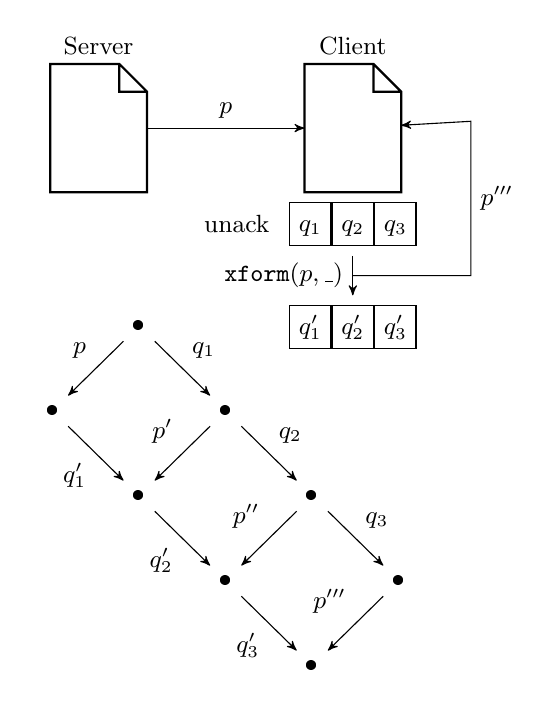
\begin{tikzpicture}[>=stealth',font=\small]
	

		\node[doc,label=above:Client] (c) {};
		\node[doc,label=above:Server\vphantom{l},left=2 of c] (s) {};
		\path[->]
			(s) edge[above] node {$p$} (c)
		;
		
		\matrix (unack) [
			below=0 of c,		
			matrix of nodes,
			every node/.style={draw},
			column sep=0em,
			label=left:unack
		]
		{
			$q_1$\vphantom{$q'_1$} & $q_2$\vphantom{$q'_1$} & $q_3$\vphantom{$q'_1$} \\
		};
		
		\matrix (unack') [
			below=.5 of unack,		
			matrix of nodes,
			every node/.style={draw},
			column sep=0em,
		]
		{
			$q'_1$ & $q'_2$ & $q'_3$ \\
		};
		
		\path[->]
			(unack) edge[left] node {$\code{xform}(p,\_)$} (unack')
		;
		\coordinate (mid) at ($ (unack)!1.0/2!(unack') $);
		\coordinate (mid') at ($ (mid) + (1.5,0) $);
		\coordinate (mid'') at ($ (mid') + (0,1.96) $);
		\draw[->] (mid) to (mid') to[right] node {$p'''$} (mid'') to (c);
			

		\matrix (m) [
			below=2.2 of $ (c)!1.0/2!(s) $,
			matrix of nodes,
			row sep=2em,
			column sep=2em,
		]
		{
			& \node (00) {\textbullet}; & \\
			\node (10) {\textbullet}; & & \node (01) {\textbullet}; \\
			&  \node (11) {\textbullet}; & & \node (02) {\textbullet}; \\
			& & \node(12) {\textbullet}; & & \node (03) {\textbullet}; \\
			& & & \node(13) {\textbullet}; \\
		};
		\path[->]
			(00) edge[above left]  node {$p$} (10)
				 edge[above right] node {$q_1$} (01)
			(01) edge[above left]  node {$p'$} (11)
				 edge[above right] node {$q_2$} (02)
			(02) edge[above left]  node {$p''$} (12)
				 edge[above right] node {$q_3$} (03)	
		;
		\path[<-]
			(13) edge[below left] node {$q'_3$} (12)
				 edge[above left] node {$p'''$} (03)
			(12) edge[below left] node {$q'_2$} (11)
			(11) edge[below left] node {$q'_1$} (10)
		;
%		\path[<-]
%			(11) edge[below left] node {$q'$} (10)
%				 edge[above left] node {$p'$} (01)
%		;
%		\path[->,dashed]
%			($ (00)!1.0/2!(10) $) edge ($ (01)!1.0/2!(11) $)
%			($ (00)!1.0/2!(01) $) edge ($ (10)!1.0/2!(11) $)
%		;
	\end{tikzpicture}
\caption{Client-side concurrency tracking.}
\label{fig:client-concurrency}
\end{figure}



%Suppose for now that any received operation $p$ 
%
%
%If the client has unacknowledged operations $q_1,\dots, q_n$, listed in the order of application, and receives an operation $p$ from the server, then the client simply applies \code{xform} 
%
%
%
%The client's local copy matches the server's master document upon initial connection.  Now suppose the client applies local operations $q_1, q_2, q_3$ in that order.  Before any are acknowledged, however, the server sends 


The server, on the other hand, must track concurrency between the operations received from many clients.  The server may simply apply operations in the order it receives; however, it must determine against which already applied operations a newly received operation should be transformed.  To do this, the server maintains a Lamport clock that corresponds to the number of operations it has applied to the master document.  The server also maintains a history of all applied operations (see Section \ref{sec:future}).  It attaches the current clock value to each broadcasted operation; then, when the client sends an operation $q$ to the server, it attaches the last received clock value from the server incremented by one.  The timestamps on the operations received by the server indicate from what point in its history it must begin transforming $q$ before applying it.

\begin{figure}
\centering
	\begin{tikzpicture}[>=stealth',font=\small]
	
		\node[doc,label=above:Server\vphantom{l}] (s) {};
		\node[doc,label=above:Client 1,right=1.8 of c] (c1) {};
		\node[doc,label=below:Client 2,below=1.2 of s] (c2) {};
	
		\path[->]
			(s.15) edge[above] node {$p_5\ p_4\ p_3\ p_2$} (c1.165)
			(c1.195) edge[below] node {$q_3$} (s.345)
		;
		\path[->]
			(s.280) edge (c2.80)
			(c2.100) edge (s.260)
		;
		
		\matrix (buf) [
			left=1 of $ (s)!1.0/6!(c2) $,
			matrix of nodes,
			every node/.style={draw},
			row sep=0 em,
			label=above:history
		]
		{
			$p_1$ \\
			$p_2$ \\
			\node[fill=black!20] (p3) {$p_3$}; \\
			\node[fill=black!20] (p4) {$p_4$}; \\
			\node[fill=black!20] (p5) {$p_5$}; \\
			\node (p6) {$p_6$}; \\
			\node[draw] (last) {\phantom{$p'_5$}}; \\
		};
		
		\coordinate (q1) at ($ (p3) + (-.6,0) $);
		\coordinate (q2) at ($ (p6) + (-.6,0) $);
		\draw[->] (q1) to[left] node {$\code{xform}(\_,q_3)$} (q2) to (p6);


		\matrix (m) [
			below=3 of $ (c1)!1.5/2!(s) $,
			matrix of nodes,
			row sep=2em,
			column sep=2em,
		]
		{
			& & & &\node (00) {\textbullet}; & \\
			& & & \node (10) {\textbullet}; & & \node (01) {\textbullet}; \\
			& & \node (20) {\textbullet}; & & \node (11) {\textbullet}; \\
			& \node(30) {\textbullet}; & & \node (21) {\textbullet}; & & \\
			& & \node(31) {\textbullet}; & & &  \\
		};
		\path[->]
			(00) edge[above left]  node {$p_3$} (10)
				 edge[above right] node {$q_3$} (01)
			(10) edge[above right]  node {$q'_3$} (11)
				 edge[above left] node {$p_4$} (20)
			(20) edge[above right]  node {$q''_3$} (21)
				 edge[above left] node {$p_5$} (30)	
		;
		\path[<-]
			(31) edge (21)
				 edge[below left] node {$q'''_3 = p_6$} (30)
			(21) edge (11)
			(11) edge (01)
		;
	\end{tikzpicture}
\caption{Server-side concurrency tracking.  The indices on the operations denote timestamps.}
\label{fig:server-concurrency}
\end{figure}

For example, consider the diagram in Figure \ref{fig:server-concurrency}, where the indices on the operations denote their timestamps.  The server has accumulated a history of 6 operations $p_1$ through $p_6$.  In the meantime, its connection with Client 1 has lagged because of network latency, such that Client 1 has just received operation $p_2$.  Client 1 then sends a new operation $q_3$.  The timestamp 3 indicates that $q_3$ applies to the same document state as $p_3$, and that all applied operations since then are concurrent with $q_3$.  Thus, the server knows to transform $q_3$ against each of the operations $p_3, p_4, p_5$.  The transformed result $q'''_3 = p_6$ is then applied to the document and added to the history.


\paragraph*{Operation composition} 
Public Record essentially supports operations of two basic types: \code{insert(i,c)}, which inserts character \code{c} at index \code{i}, and \code{delete(i)}, which deletes the character at index \code{i}.  However, actually representing operations at this level of granularity is not optimal. Recall that the client must wait until each local operation is acknowledged by the server before it sends another.  Sending out operations on individual characters in this fashion may cause unacceptably slow rates of convergence between users in the presence of network latency.  
%In the presence of any nontrivial network latency, this could induce a vicious cycle: the client must wait longer than usual to send out operations, during which the user applies more changes, thereby causing the client to take even longer to send out operations, and so on.

To optimize against this, we borrow a trick from Google \cite{S} and structure operations so that they support \emph{composition}.  With operation composition, a client may simply compose together any local operations that occur while it waits for another to be acknowledged.  We elaborate on this optimization further below.
%that are applied between the sending and acknowledgement of an operation.  
%For example, in Figure \ref{fig:composition}, the client may compose together the operations $q_2, q_3, q_4$ into $q$ while waiting for acknowledgment of $q_1$.

%\begin{figure}
%\centering
%	\begin{tikzpicture}[>=stealth',font=\small]
%	
%		\node[doc,label=above:client] (c) {};
%		
%		\matrix (m) [
%			below=0 of c,		
%			matrix of nodes,
%			every node/.style={draw},
%			column sep=0em,
%			label=left:unack
%		]
%		{
%			\node(q1){$q_1$\vphantom{$q'_1$}}; & \node(q2){$q_2$\vphantom{$q'_1$}}; & \node(q3){$q_3$\vphantom{$q'_1$}}; & \node(q4){$q_4$\vphantom{$q'_1$}}; \\
%		};
%		
%		\draw[decorate,decoration={brace,mirror,raise=2pt}]
%			(q2.south west) --node[below=.2cm]{$q$} (q4.south east)
%		;
%	\end{tikzpicture}
%\caption{Optimization via operation composition.}
%\label{fig:composition}
%\end{figure}

To support composition, operations are structured as \emph{traversals} of the whole document.  Specifically, an operation is an ordered list containing primitive traversal units of three types:
\begin{itemize}
\item \code{retain(n)} for some integer \code{n}, which advances the current position within the document by \code{n} characters;
\item \code{insert(s)} for some string \code{s}, which inserts the string \code{s} at the current position, then advances the current position by the length of \code{s};
\item \code{delete(n)} for some integer \code{n}, which deletes the next \code{n} characters from the current position.
\end{itemize}
In this form, an insertion that changes the document from \code{abc} to \code{abxc} would be represented as \code{retain(2),insert(x),retain(1)}.  

Now consider Figure \ref{fig:composition-example}, which depicts a client's buffer of unacknowledged operations.  Figure \ref{fig:composition-example-a} shows the buffer at the granularity of individual character insertions and deletions.  While the client waits for acknowledgment of the first operation \code{ret(10),ins(s)}, however, it may compose the remaining operations in its buffer to a single operation as shown in Figure \ref{fig:composition-example-b}.  In so doing, the client minimizes the number of operations it must send to the server.

\begin{figure}
\centering
	\begin{subfigure}{\linewidth}
	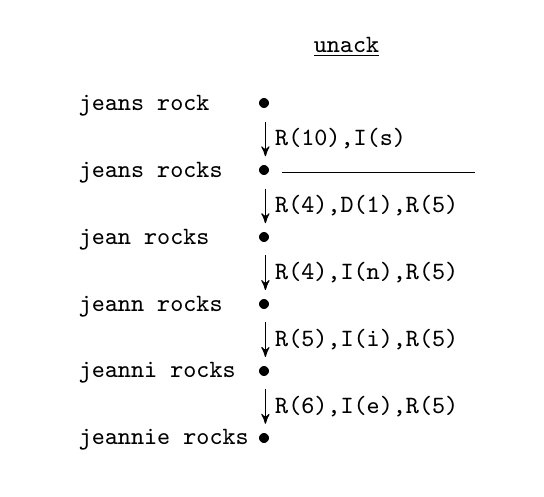
\begin{tikzpicture}[>=stealth',font=\ttfamily\small]
		\matrix (m) [
			matrix of nodes,
%			every node/.style={inner sep=0pt},			
			row sep=1em,
			column sep=-.3em,
		]
		{
			\node[label=right:jeans rock] {\phantom{\textbullet}}; & \textbullet  \\
			\node[label=right:jeans rocks] {\phantom{\textbullet}}; & \node (b) {\textbullet};\node[label=right:\phantom{R(4),D(1),R(5)}] {\phantom{\textbullet}}; & \node (c) {\phantom{\textbullet}}; \\
			\node[label=right:jean rocks] {\phantom{\textbullet}}; & \textbullet \\
			\node[label=right:jeann rocks] {\phantom{\textbullet}}; & \textbullet \\
			\node[label=right:jeanni rocks] {\phantom{\textbullet}}; & \textbullet \\
			\node[label=right:jeannie rocks] {\phantom{\textbullet}}; & \textbullet \\
%			\node[label=left:jeans rock] {\textbullet}; \\
		};
		\path[->]
			(m-1-2) edge[right] node {R(10),I(s)} (b)
			(b) edge[right] node {R(4),D(1),R(5)} (m-3-2)
			(m-3-2) edge[right] node {R(4),I(n),R(5)} (m-4-2)
			(m-4-2) edge[right] node {R(5),I(i),R(5)} (m-5-2)
			(m-5-2) edge[right] node {R(6),I(e),R(5)} (m-6-2)
		;
		\path (b) edge (c) ;
		\node[above right=.4 of m-1-2] {\underline{unack}};
	\end{tikzpicture}
	\caption{}
	\label{fig:composition-example-a}
	\end{subfigure}	
	\vspace{.5cm}
	
	\begin{subfigure}{\linewidth}
	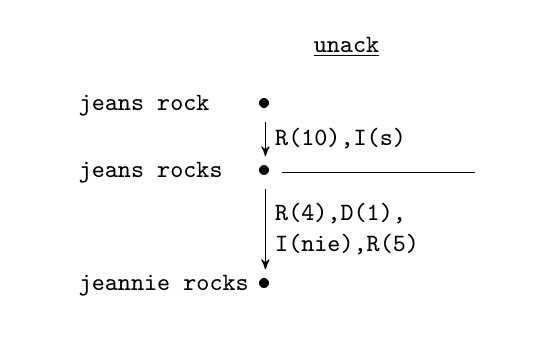
\begin{tikzpicture}[>=stealth',font=\ttfamily\small]	
		\matrix (m) [
			matrix of nodes,
			row sep=1em,
			column sep=-.3em		
		]
		{
			\node[label=right:jeans rock] {\phantom{\textbullet}}; & \textbullet  \\
			\node[label=right:jeans rocks] {\phantom{\textbullet}}; & \node (b) {\textbullet};\node[label=right:\phantom{R(4),D(1),R(5)}] {\phantom{\textbullet}}; & \node (c) {\phantom{\textbullet}}; \\
%			\node[label=right:jean rocks] {\phantom{\textbullet}}; & {} \\
%			\node[label=right:jeann rocks] {\phantom{\textbullet}}; & {} \\
%			\node[label=right:jeanni rocks] {\phantom{\textbullet}}; & {} \\
			{} & {} \\
			\node[label=right:jeannie rocks] {\phantom{\textbullet}}; & \textbullet \\
%			\node[label=left:jeans rock] {\textbullet}; \\
		};
		\path[->]
			(m-1-2) edge[right] node {R(10),I(s)} (b)
			(b) edge[right,text width=2cm] node {R(4),D(1),\\ I(nie),R(5)} (m-4-2)
		;
		\path (b) edge (c) ;
		\node[above right=.4 of m-1-2] {\underline{unack}};
	\end{tikzpicture}
	\caption{}
	\label{fig:composition-example-b}
	\end{subfigure}
\caption{A client's buffer of unacknowledged operations (a)  without composition and (b) with composition.%$^{please^{love^{us}}}$
}
\label{fig:composition-example}
\end{figure}



\section{Evaluation} \label{sec:evaluation}

\section{Future Work} \label{sec:future}

There are many obvious directions for future work on Public Record.  One glaring implementation flaw is our lack of maintenance of the server's queue that stores the history of all applied operations.  This could easily be managed by keeping track of last-received operation timestamps for each client, and removing from the queue any operations with timestamps smaller than any client.  Without this fix, Public Record is certain to run out of memory if it runs for long enough.  A related improvement would be to replicate the master document to ensure that it truly persists.


\begin{thebibliography}{S} % '2nd argument contains the widest acronym'

\bibitem[S]{S}  D.\ Spiewak. ``Understanding and Applying Operational Transformation''. 17 May 2010. [Blog entry]. Code Commit. Available \url{http://www.codecommit.com/blog/java/understanding-and-applying-\\ operational-transformation}\newline [Accessed: 20 May 2016]


%D. Lacey. ?Reflections on Infosecurity Europe Week?. 28 Apr 2012. [Blog entry]. David Lacey?s IT Security Blog. Available http://www.computerweekly.com/blogs/david_lacey/2012/04/reflections_on_infosecurity_eu_2.html [Accessed: 30 Apr 2012]

\end{thebibliography}




\end{document}
